\documentclass[12pt]{standalone}

\usepackage{tikz}
\usepackage{ctex}

\begin{document}
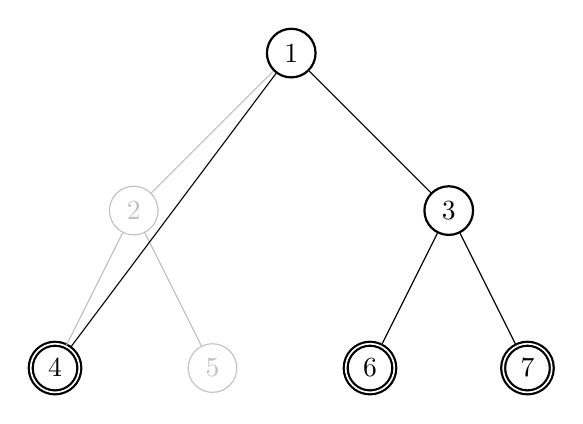
\begin{tikzpicture}
    [level distance=2cm,
    level 1/.style={sibling distance=4cm},
    level 2/.style={sibling distance=2cm}]

    \scoped[color=lightgray,every node/.style={circle,draw}]
    \node[color=black,thick] (A) at (0,0) {$1$}
        child {node (B) {$2$}
            child {node[color=black,double,thick] (D) {$4$}}
            child {node (E) {$5$}}}
        child {node[color=black,thick] (C) {$3$}
            child {node[color=black,double,thick] (F) {$6$}}
            child {node[color=black,double,thick] (G) {$7$}}};

    \draw (A) -- (D);
    \draw (A) -- (C);
    \draw (C) -- (F);
    \draw (C) -- (G);

\end{tikzpicture}
\end{document}
